
%% bare_conf.tex
%% V1.4b
%% 2015/08/26
%% by Michael Shell
%% See:
%% http://www.michaelshell.org/
%% for current contact information.
%%
%% This is a skeleton file demonstrating the use of IEEEtran.cls
%% (requires IEEEtran.cls version 1.8b or later) with an IEEE
%% conference paper.
%%
%% Support sites:
%% http://www.michaelshell.org/tex/ieeetran/
%% http://www.ctan.org/pkg/ieeetran
%% and
%% http://www.ieee.org/

%%*************************************************************************
%% Legal Notice:
%% This code is offered as-is without any warranty either expressed or
%% implied; without even the implied warranty of MERCHANTABILITY or
%% FITNESS FOR A PARTICULAR PURPOSE! 
%% User assumes all risk.
%% In no event shall the IEEE or any contributor to this code be liable for
%% any damages or losses, including, but not limited to, incidental,
%% consequential, or any other damages, resulting from the use or misuse
%% of any information contained here.
%%
%% All comments are the opinions of their respective authors and are not
%% necessarily endorsed by the IEEE.
%%
%% This work is distributed under the LaTeX Project Public License (LPPL)
%% ( http://www.latex-project.org/ ) version 1.3, and may be freely used,
%% distributed and modified. A copy of the LPPL, version 1.3, is included
%% in the base LaTeX documentation of all distributions of LaTeX released
%% 2003/12/01 or later.
%% Retain all contribution notices and credits.
%% ** Modified files should be clearly indicated as such, including  **
%% ** renaming them and changing author support contact information. **
%%*************************************************************************


% *** Authors should verify (and, if needed, correct) their LaTeX system  ***
% *** with the testflow diagnostic prior to trusting their LaTeX platform ***
% *** with production work. The IEEE's font choices and paper sizes can   ***
% *** trigger bugs that do not appear when using other class files.       ***                          ***
% The testflow support page is at:
% http://www.michaelshell.org/tex/testflow/
\documentclass[conference]{IEEEtran}
\usepackage{hyperref}
\usepackage{enumitem}
\usepackage{amssymb}
\usepackage{amsmath}
\usepackage{algorithmicx}
\usepackage{algorithm}
\usepackage{algpseudocode}
\usepackage{graphicx}
\usepackage{subfigure}


\begin{document}
%
% paper title
% Titles are generally capitalized except for words such as a, an, and, as,
% at, but, by, for, in, nor, of, on, or, the, to and up, which are usually
% not capitalized unless they are the first or last word of the title.
% Linebreaks \\ can be used within to get better formatting as desired.
% Do not put math or special symbols in the title.
\title{Monte Carlo Tree Search with Options\\for General Video Game Playing}


% author names and affiliations
% use a multiple column layout for up to three different
% affiliations
\author{\IEEEauthorblockN{Maarten de Waard}
\IEEEauthorblockA{University of Amsterdam\\
Science Park 904\\
Amsterdam, Netherlands\\
Email: \href{mailto:mrtndwrd@gmail.com}{mrtndwrd@gmail.com}}
\and
\IEEEauthorblockN{Diederik M. Roijers}
\IEEEauthorblockA{Oxford University\\
???\\
Email: \href{mailto:???}{???}}
\and
\IEEEauthorblockN{Sander C.J. Bakkes}
\IEEEauthorblockA{Tilburg University\\
Warandelaan 2, Dante Building\\
Tilburg, Netherlands\\
Email: \href{mailto:S.C.J.Bakkes@uvt.nl}{S.C.J.Bakkes@uvt.nl}}
}

% conference papers do not typically use \thanks and this command
% is locked out in conference mode. If really needed, such as for
% the acknowledgment of grants, issue a \IEEEoverridecommandlockouts
% after \documentclass

% for over three affiliations, or if they all won't fit within the width
% of the page, use this alternative format:
% 
%\author{\IEEEauthorblockN{Michael Shell\IEEEauthorrefmark{1},
%Homer Simpson\IEEEauthorrefmark{2},
%James Kirk\IEEEauthorrefmark{3}, 
%Montgomery Scott\IEEEauthorrefmark{3} and
%Eldon Tyrell\IEEEauthorrefmark{4}}
%\IEEEauthorblockA{\IEEEauthorrefmark{1}School of Electrical and Computer Engineering\\
%Georgia Institute of Technology,
%Atlanta, Georgia 30332--0250\\ Email: see http://www.michaelshell.org/contact.html}
%\IEEEauthorblockA{\IEEEauthorrefmark{2}Twentieth Century Fox, Springfield, USA\\
%Email: homer@thesimpsons.com}
%\IEEEauthorblockA{\IEEEauthorrefmark{3}Starfleet Academy, San Francisco, California 96678-2391\\
%Telephone: (800) 555--1212, Fax: (888) 555--1212}
%\IEEEauthorblockA{\IEEEauthorrefmark{4}Tyrell Inc., 123 Replicant Street, Los Angeles, California 90210--4321}}




% use for special paper notices
%\IEEEspecialpapernotice{(Invited Paper)}



\maketitle
\begin{abstract}
	Many decision-theoretic algorithms are used in general video game playing,
	because they are highly effective problem solvers.  ``Monte Carlo Tree
	Search'' (MCTS) is a popular decision-theoretic algorithm that has often
	been used for general video game playing.  The MCTS algorithm always plans
	over actions and does not incorporate any high level planning, as one would
	expect from a human player. Furthermore, although many games have similar
	game dynamics, often no prior knowledge is available to general video game
	playing algorithms.  In this paper, we introduce a new algorithm called
	``Option Monte Carlo Tree Search'' (O-MCTS). It offers general video game
	knowledge and high level planning in the form of options, which are action
	sequences aimed at achieving a specific subgoal. Additionally, we introduce
	``Option Learning MCTS'' (OL-MCTS), which applies a progressive widening
	technique to the expected returns of options in order to focus exploration
	on fruitful parts of the search tree. Our new algorithms are compared to
	MCTS on a diverse set of twenty-eight games from the general video game AI
	competition. Our results indicate that by using MCTS's efficient tree
	searching technique on options, O-MCTS outperforms MCTS on most of the
	games, especially those in which a certain subgoal has to be reached before
	the game can be won.  Lastly, we show that OL-MCTS improves its performance
	on specific games by learning expected values for options and moving a bias
	to higher valued options.
\end{abstract}

% A category with the (minimum) three required fields
%\category{H.4}{Information Systems Applications}{Miscellaneous}
%A category including the fourth, optional field follows...
%\category{D.2.8}{Software Engineering}{Metrics}[complexity measures, performance measures]

%\terms{Theory}

%\keywords{MCTS, GVGAI, general video game AI, options, macro-actions}

\section{Introduction}
\label{sec:introduction}

An increasingly important goal in decision theory is creating AI algorithms that
are capable of solving more than one problem. A general AI, instead of a
specific alternative, is considered a step towards creating a strong AI.  An
especially challenging domain of AI is general video game playing.  Since many
real-world problems can be modeled as a game, algorithms that can play complex
games successfully are often highly effective problem solvers in other areas.
Although decision theory and general video game playing are different research
areas, both can benefit from each other.  An increase in performance in general
video game playing can be found by using algorithms designed for complex
decision-theoretic problems, whereas the algorithms that are created for general
video game playing can be applied to other decision-theoretic problems.
Furthermore, applying decision-theoretic algorithms to a new class of problems,
like general video game playing, can lead to a better understanding of the
algorithms, and new insights in their strengths and weaknesses. 

% TODO: Move this further?
Recent research focusses on algorithms capable of solving several games with
different types of objectives. A common approach is to use a tree search in
order to select the best action for any given game state. In every new game
state, the tree search is restarted until the game ends.  A popular example is
\emph{Monte Carlo tree search (MCTS)}.

A method to test the performance of a general video game playing algorithm is
by using the framework of the \emph{general video game AI (GVGAI)} competition
\cite{perez2014}. In this competition, algorithm designers can test their
algorithms on a set of diverse games. When submitted to the competition, the
algorithms are applied to an unknown set of games in the same framework to test
their general applicability. Many of the algorithms submitted to this contest
rely on a tree search method.

A limitation in tree search algorithms is that since many games are too complex
to plan far ahead in a limited time frame, many tree algorithms incorporate a
maximum search depth. As a result, tree search based methods often only
consider short-term score differences and do not incorporate long-term
plans. Moreover, many algorithms lack common video game knowledge and do not
use any of the knowledge gained from the previous games.

In contrast, when humans play a game we expect them to do assumptions about its
mechanics, e.g., pressing the left button often results in the player's avatar
moving to the left on the screen. Players can use these assumptions to learn how
to play a game more quickly. Furthermore, human players are able to have an
abstraction layer over their action choices; instead of choosing one action at a
time they define a specific subgoal for themselves: when there is a portal on
screen, a human player is likely to try to find out what the portal does by
walking towards its sprite (the image of the portal on the screen). The player
will remember the effect of the portal sprite, and use that information for the
rest of the game. In this case, walking towards the portal can be seen as a
subgoal of playing the game.

In certain situations, it is clear how such a subgoal can be achieved and a
sequence of actions, or \emph{policy}, can be defined to achieve it. A policy to
achieve a specific subgoal is called an option \cite{sutton1999between}. Thus, an option selects an 
action, given a game state, that aims at satisfying its subgoal. Options, in
this context, are game-independent. For example, an option that has reaching a
specific location in the game (for example a portal) as its objective selects
actions using a path planning heuristic that will reach the goal location. 
The probability of this kind of subgoal being achieved by an algorithm that
does not use options is smaller, especially when the road to the subgoal does
not indicate any advantage for the player. For instance, in the first few
iterations of MCTS, the algorithm will be equally motivated to move 10 steps
into the direction of a certain game sprite as it will be to do any other
combination of 10 actions. 

Therefore, we propose a new algorithm called \emph{option Monte Carlo tree
search (O-MCTS)} that extends MCTS to use options. Because O-MCTS chooses
between options rather than actions when playing a game, we expect it to be able
to plan at a higher level of abstraction. Furthermore, we introduce \emph{option
learning MCTS (OL-MCTS)}, an extension of O-MCTS that approximates which of the
options in the option set is more feasible for the game it is playing. This can
be used to shift the focus of the tree search exploration to more promising
options. This information can be transferred in order to increase performance on
the next level.

The new algorithms are benchmarked against MCTS on games from the General Video
Game AI competition. Our results indicate that the O-MCTS and OL-MCTS algorithms
outperform MCTS in games that require a high level of action planning, e.g.,
games in which something has to be picked up before a door can be opened. In
most other games, O-MCTS and OL-MCTS perform at least as good as MCTS.


\chapter{Background}
\label{sec:background}

This chapter explains the most important concepts needed to understand the
algorithms that are proposed in this thesis. We first describe \emph{Markov
decision processes (MDPs)}, the type of problem that our algorithms have to
deale with. Then  MCTS the tree search algorithm that is commonly used on MDPs.
Subsequently, options will be explained, these simulate the idea of defining
subgoals and reaching them.  Then, the basics of Q-learning are described.
Finally the \emph{video game description language (VGDL)} is explained. This is
the protocol that is used in the GVGAI competition to generate many different
games that all have the same interaction with the game playing algorithms.

\section{Markov Decision Processes}
\label{subsec:mdps}
In this thesis, each game will be treated as an MDP. MDPs provide a mathematical
framework for use in decision making problems. An MDP is formally defined as a
tuple $\langle S, A, T, R \rangle$. $S$ denotes the set of states. An MDP is
fully observable, meaning that a state contains all the information of the
game's current condition: locations of monsters, the avatar, etc. $A$ is a
finite set of actions, the input an agent can deliver to the game. $T$ is a
transition function defined as $T : S \times A \times S \rightarrow
\left[0,1\right]$. It specifies the probabilities over the possible next states,
when taking an action in a state.  $R$ is a reward function defined as $R: S
\times A \times S \rightarrow \mathbb{R}$. In this case, when the game score
increases, the increase is viewed as the reward. Algorithms typically maximize
the cumulative reward, which is analogous to the score. An MDP by definition has
the \emph{Markov property}, which means that the conditional probability
distribution of future states depends only upon the present state. No
information from previous states is needed. Algorithms do not have access to $T$
and $R$ in the scope of this thesis.

For example, for the game Zelda, a state $s$ consists of the location, rotation
and speed of the avatar, the location of the monsters, the locations of walls
and the location of the key and portal that need to be found. $S$ is the set of
all possible states, so all possible combinations of these variables. The action
set $A$ consists of the actions \textsc{up}, \textsc{down}, \textsc{left},
\textsc{right} and \textsc{use}. The transition function $T$ defines the
transition from a state, given an action. This means that the transition defines
the change in location of the monsters and the avatar, if any of the sprites
disappear (like when the avatar picks up the key), etc. Note that, since the
transition function is not by definition deterministic, the resulting state from
an action $a$ in state $s$ is not always the same state. For example: because a
monster moves about randomly, it could have moved left or right in the new
state. The reward function describes the change in game score, given a state,
action and resulting next state, for example when the avatar kills a monster
with the action \textsc{use}, its score will increase with 1.

\section{Monte Carlo Tree Search}
\begin{figure}
	\centering
	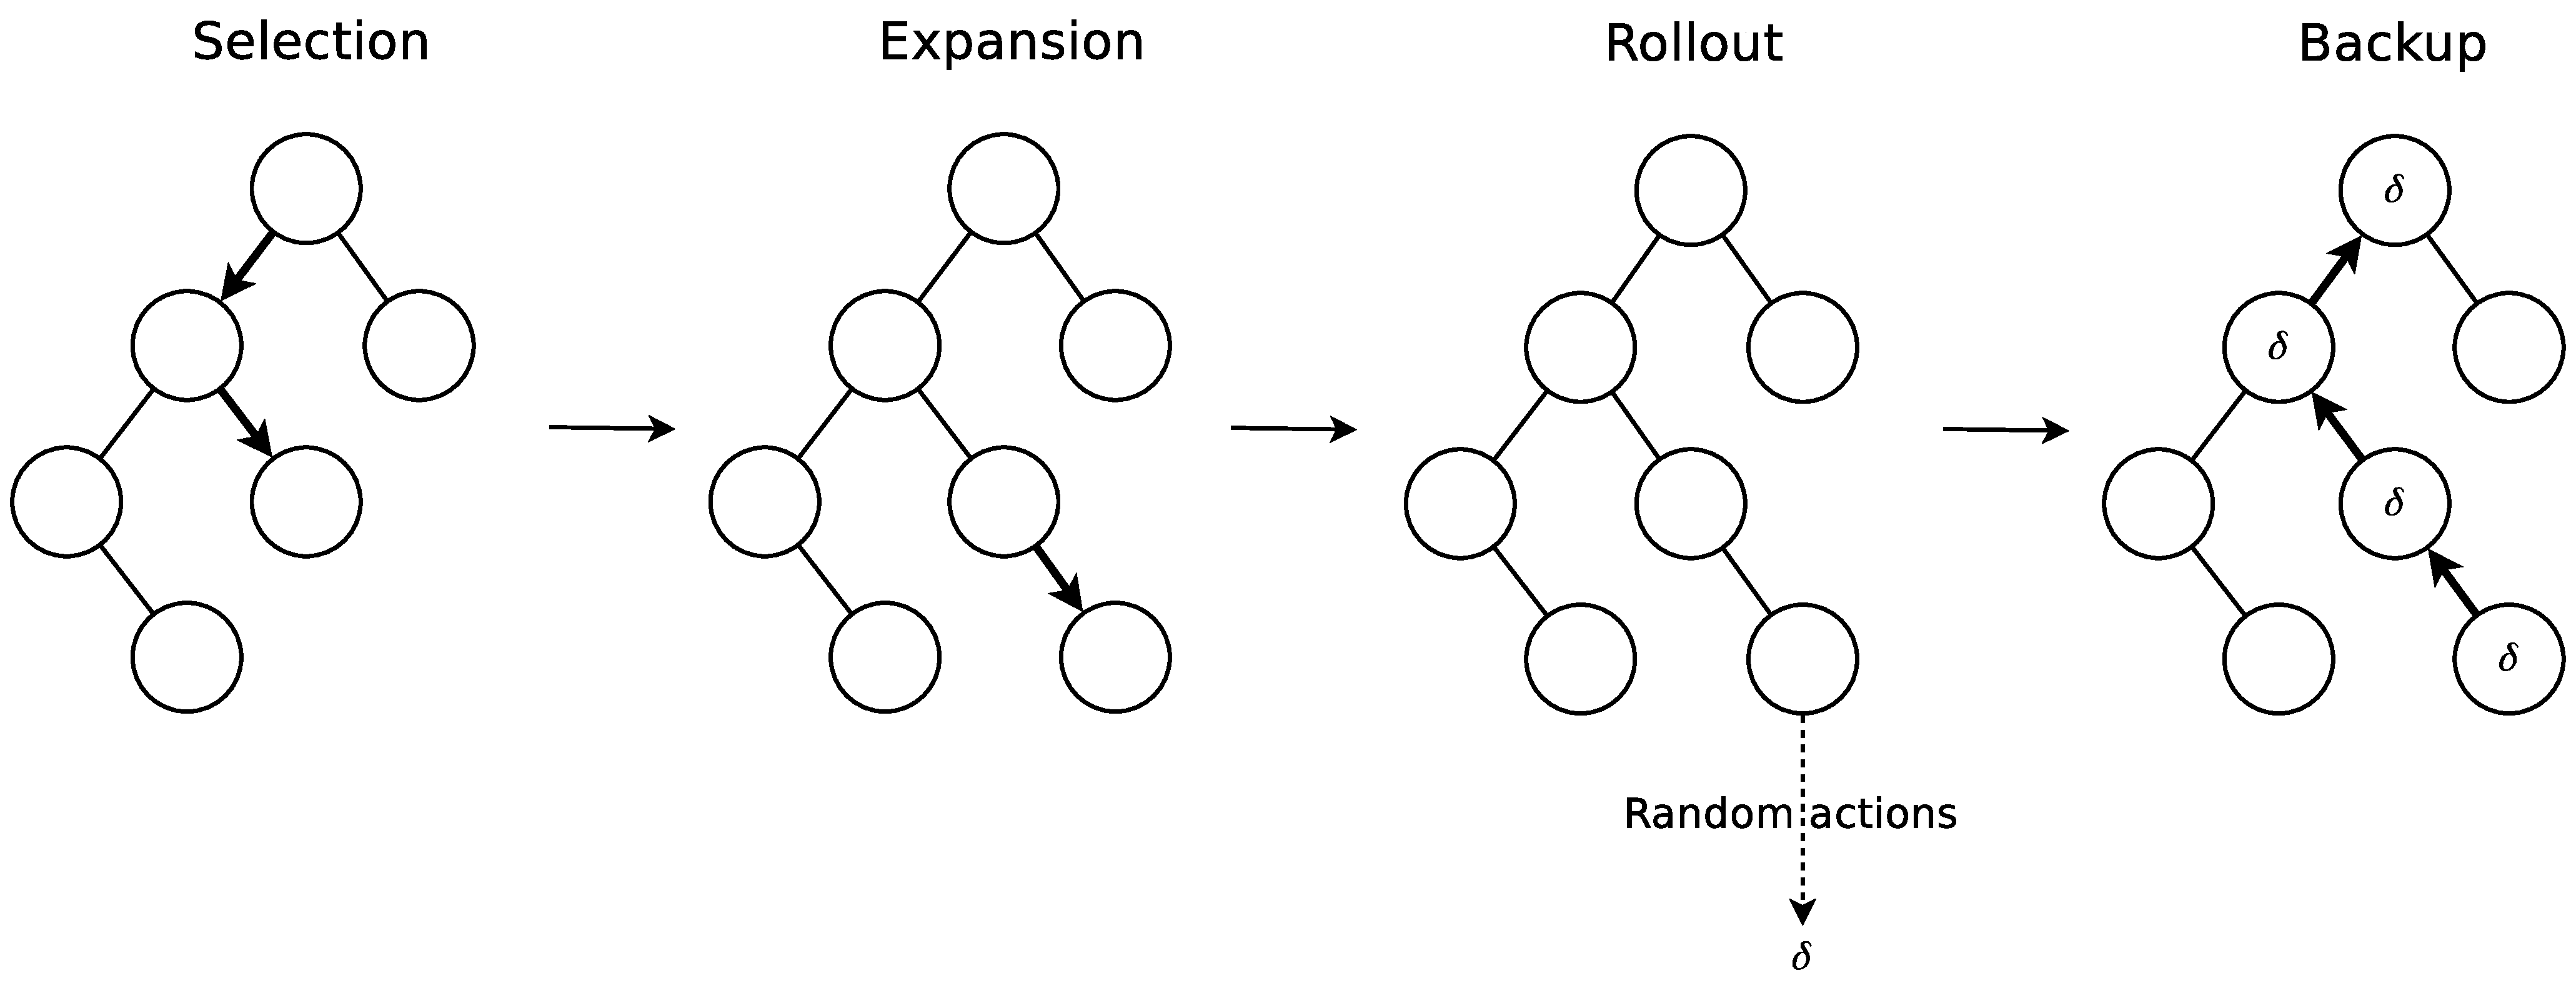
\epsfig{file=includes/mcts-wide.eps, width=\textwidth}
	\caption{One Monte Carlo tree search iteration}
	\label{fig:mcts}
\end{figure}

\label{subsec:mcts}
Monte Carlo methods have their roots in statistical physics, where they have
been used to approximate intractable integrals. Abrahamson
\cite{abramson1990expected} demonstrated theoretically that this sampling method
might be useful for action selection in games as well.  In 2001, Monte Carlo
methods were effectively used for bridge \cite{ginsberg2001gib}. The real
success of MCTS started in 2006, when the tree search method and UCT formula
were introduced, yielding very good results in Computer Go
\cite{gelly2006modification}. Since 2006, the algorithm has been extended with
many variations is still being used for other computer games
\cite{browne2012survey}, including the GVGAI competition
\cite{perez2014knowledge}.

This section explains how it approximates the value of actions taken in a
specific state. A tree is built incrementally from the states and actions that
are visited in a game. Each node in the tree represents a state, each connection
in the tree represents an action taken in that state leading to a state, which
is represented by the next tree node.  The process, as explained in Figure
\ref{fig:mcts}, consists of four phases that are constantly repeated. It is
started with the current game state, which is represented by the root node of
the tree. The first action is chosen by an \emph{expansion strategy} and
subsequently simulated, resulting in a new game state, for which a new node is
created. A \emph{rollout} is done from the new node, which means that a
simulation is run from the new node applying random actions until a predefined
stop criterion is met or the game ends. Finally, the score difference resulting
from the rollout is backed up, to the root node, which means that the reward is
saved to the visited nodes. Then a new iteration starts. When all actions are
expanded in a node, we call that node \emph{fully expanded} and use a
\emph{selection strategy} to select a next node. When a node is selected that is
not fully expanded, the expansion strategy is used to create a new node, after
which a rollout takes place and the results are backed up thereafter.

	%(Term from pMCTS.pdf)
The selection strategy selects optimal actions in internal tree nodes, depending
on the values of the child nodes. An effective and very popular selection
strategy is the \emph{upper confidence tree (UCT)} \cite{kocsis2006bandit},
which balances the choice between poorly explored actions with a high
uncertainty about their value and actions that have been explored but have a
higher value. A child node $j$ is selected to maximize
\begin{equation}
	\label{eq:uct}
	UCT = 2C_p \sqrt{\frac{2 \ln n_s}{n_{s'}}}
\end{equation}
Where $n_s$ is the number of times the current node $s$ has been visited,
$n_{s'}$ is the number of times child $c$ has been visited and $C_p > 0$ is a
constant, often set to $\sqrt{2}$, that shifts priority from exploration to
exploitation.

The traditional expansion strategy is to explore each action at least once in
each node. After all actions have been expanded, the node applies the selection
strategy for further exploration. Some variants of MCTS reduce the branching
factor of the tree by only expanding the nodes selected by a special expansion
strategy. A specific example is the \emph{crazy stone} algorithm
\cite{coulom2007efficient}, which is an expansion strategy that was designed
specifically for Go. We will use an adaptation of this strategy in the algorithm
proposed in Section \ref{sec:learning}.  When using crazy stone, an action $i$
is selected with a probability proportional to $u_i$
\begin{equation}
	\label{eq:crazystone}
	u_i = \exp\left(K \frac{\mu_0 - \mu_i}{\sqrt{2\left(\sigma_0^2 +
\sigma_i^2\right)}}\right) + \epsilon_i
\end{equation}
Each action has an estimated value $\mu_i$ ordered in such a way that $\mu_0 >
\mu_1 > \ldots > \mu_N$, and a variance $\sigma_i^2$. $\epsilon_i$ prevents 
the probability of selecting a move to reach zero and its value is proportional to
the ordering of the expected values of the possible actions. K is a constant
that influences the exploration/exploitation trade off.
\begin{equation}
	\label{eq:epsilon}
	\epsilon_i = \frac{0.1 + 2^{-i} + a_i}{N}
\end{equation}
Where $a_i$ is 1 when an action is \emph{an atari move}, a go-specific
move that can otherwise easily be underestimated by MCTS, and otherwise 0.

After a rollout, the reward is backed up, which means that the estimated value
for every node that has been visited in this iteration is updated with the
reward of this simulation. Usually the estimated value of a node is the average
of all rewards backed up to that node.

\section{Q-learning}
\label{subsec:qlearning}
Q-learning is a relatively simple model free temporal difference learning method
that was proposed in 1992 \cite{watkins1992q}. The \emph{Q-value}, $Q(s, a)$, is
the discounted reward that can be achieved by applying action $a$ to state $s$
and following the optimal policy afterwards. By learning Q-values for every
action in every state, it can estimate an optimal policy. 

The general idea of Q-learning is to incrementally save the reward from the MDP,
in combination with the current Q-value function: the update function uses the
reward and the maximum of the Q-values of the next state: 
\begin{equation}
	\label{eq:qlearning}
	Q(s, a) \gets Q(s, a) + \alpha \left(r + \gamma \max_a Q(s', a) - Q(s, a)\right),
\end{equation}
where $r$ is the reward that is achieved by using action $a$ in state $s$,
leading to state $s'$. The algorithm has two parameters: $\gamma$ is the
discount factor. This indicates the importance of future states. $\alpha$ is the
learning rate, which determines how quickly the Q-values are updated. An
exploration policy selects the actions for each state.  The Q-table can be used
to find the optimal policy by, for each state $s$, selecting the action $a$ that
maximizes $Q(s, a)$. Because after each action only one state-action pair is
being updated, Q-learning can take a long time to converge, but it is guaranteed
to converge to the optimal policy, given that the exploration policy visits each
state-action pair an infinite number of times and, for stochastic problems, the
learning rate $\alpha$ decreases over time.

\section{Options}
\label{subsec:options}
For mimicking human game playing strategies like defining and solving subgoals
and subtasks, we use options \cite{sutton1999between, barto2003recent}. An
option is a predefined method of reaching a specific subgoal. Formally, it is a
triple $\langle I, \pi, \beta\rangle$ in which $I \subseteq S$ is an initiation
set, $\pi: S \times A \rightarrow [0, 1]$ is a policy and $\beta: S^+
\rightarrow[0,1]$ is a termination condition.

A policy $\pi$ defines the action that should be taken in a state. The
initiation set $I$ is a set of states in which the option can be started. When the
option starts, policy $\pi$ will be followed, until a state is reached that
satisfies a termination condition in $\beta$. Using options in an MDP removes
the Markov property for that process: the state information alone is no longer
enough to predict an agent's actions, since the actions are now not only
state-dependant, but dependant on what option the agent has chosen in the past
as well. According to \cite{sutton1999between}, we can now view the process as
a \emph{semi-Markov decision process (SMDP)} \cite{duff1995reinforcement},
since its actions are of variable length. For convenience, we will call the
original action set of the MDP $A$, and the set of options $O$.  Normal actions
can be treated as options as well.  An option for action $a \in A$ has a
initiation set $I = S$, the policy $\pi$ is taking action $a$ in all the
states.  The termination condition $\beta$ is that action $a$ should be
performed once.


\section{Video Game Description Language}
\label{subsec:vgdl}
This thesis will use a framework called the video game description
language \cite{schaul2013video}, in which games can very easily be defined.

To define a game in VGDL, two files should be created. Firstly, the game
description should be made, which defines for each type of object what its
character in the level description is, what it looks like in the game, how it
interacts with other objects and the world, and when it disappears from the
game. Secondly, a level description should be made, in which each character maps
to an object in the game, on the same grid location as the character has in the
file. By only defining these two files a wide spectrum of games can be created.

In this thesis, we will use a Java implementation made for the GVGAI competition,
which comes with many games. The algorithm proposed in this thesis will be
benchmarked on these games, using the rules of the GVGAI competition. 


\chapter{Related Work}
\label{sec:related}
This chapter covers some popular alternative methods for general video game
playing and prior work on tree search with options. \emph{Deep Q networks (DQN)}
is a popular algorithm that trains a convolutional neural network for a game
\cite{mnih2013playing}, \emph{Planning under Uncertainty with Macro-Actions
(PUMA)} is a forward search algorithm that uses extended actions in
\emph{partially observable MDPs (POMDPs)} \cite{he2010puma}.  \emph{Purofvio} is
an algorithm that combines MCTS with macro-actions that consist of repeating one
action several times \cite{powley2012monte}. 

DQN is a general video game playing algorithm that trains a convolutional neural
network that has the last four pixel frames of a game as input and tries to
predict the return of each action. A good policy can then be created by
selecting the action with the highest return. This is one of the first
algorithms that successfully combines neural network learning with reinforcement
learning. In this case, however, it was not desirable to implement DQN because
of the limitations proposed by our testing framework. The GVGAI competition
framework currently works best for planning algorithms, that use the forward
model to quickly find good policies. Learning over the course of several games
is difficult. In contrast, DQN typically trains on one game for several days
before a good policy is found and does not utilize the forward model, but always
applies actions directly to the game in order to learn.

There are, however, examples of other learning algorithms that have been successfully
implemented in the GVGAI framework. These 
algorithms can improve their scores after playing a game for several times,
using a simple state representation \cite{samothrakis2015neuroevolution}. Their
features consist of: 
\begin{itemize}%[noitemsep]
	\item the game score, 
	\item the game tick,
	\item the winner ($-1$ if game is still ongoing, $0$ if the player lost and
		$1$ if the player won), 
	\item game over ($0$ if the game is ongoing, $1$ if the game is over), 
	\item a list of resources, 
	\item a list of Euclidean distances to the nearest sprite of each type,
	\item the speed of the avatar. 
\end{itemize}
The results of the paper show that the algorithms are capable of learning in the
course of 1000 game plays of the first level of each game. It has to be noted
that no results of how many times the algorithms \emph{win} the game are
reported and that it seems (looking at the score that is achieved) that many of
the games are actually lost most of the times. The learning algorithms proposed
in this thesis will focus more on early results than on long term learning.

An alternative tree search algorithm is PUMA, which applies forward search to
options (referred to as macro-actions) and works on POMDPs, which means it does
not restrict an MDP to be fully observable.  PUMA automatically generates
goal-oriented MDPs for specific subgoals. The advantage of this is that
effective options can be generated without requiring any prior knowledge of the
(PO)MDP. The disadvantage is that this takes a lot of computation time and thus
would not work in the GVGAI framework, in which only a limited amount of
computation time is allowed between actions. Options generated for one game,
would not necessarily be transferable to other games, meaning that option
generation would have to be done prior to every game that the algorithm plays.
Furthermore, PUMA has to find out the optimal length per macro-action, whereas
the algorithms proposed in this thesis can use options of variable length.

Another algorithm that uses MCTS with macro actions is called Purofvio.
Purofvio plans over macro-actions which, in this case, are defined as repeating
one action for a fixed number of times. No more complex options are defined.
The algorithm is constructed for the physical traveling salesperson problem,
which offers the same type of framework as the GVGAI competition: a simulator is
available during limited action time, after which an action has to be returned.
An important feature of this algorithm is that it can use the time budget of
several actions to compute which macro-action to choose next.  This is possible
because a macro-action is not reconsidered after it has been chosen. The paper
notes that their options must always be of the same length, because they found
that otherwise MCTS seems to favor options with a longer time span over shorter
options. It is suggested that Purofvio could work on other games as well, but
this has not been shown.


\section{Planning}
\label{sec:planning}
This section will explain how MCTS has to be adjusted in order to be able to
plan over options in stead of actions. 

As in normal MCTS the tree building starts at a root node, which represents the
current game state $s \in S$. An option set $O_s$ is constructed from all the
options that have state $s$ in their initiation set $I$. The expansion
strategy then choses an option. The option selects an action $a$ according to its
policy $\pi(s)$ for this state, after which a new child node is created for the
new state $s'$. Then, a rollout is done, first completing the option and
afterwards applying random actions. The results of the rollout are backed up to
the visited node and the algorithm starts over at the root node.

%\begin{wrapfigure}{r}{0.45\textwidth}
%	\begin{minipage}{0.45\textwidth}
%		\vspace{-22pt}
		\begin{algorithm}[H]
			\caption{$\mathsf{O-MCTS}(s, t, mt)$}
			\label{alg:omcts}
			\begin{algorithmic}[1]
			%\Require Initial queue $Q$, integer $k$
			%\State $P \gets \emptyset$ \textit{$\blacktriangleleft$ the Pareto archive} \label{alg:qpls:init}

			\While {$t < mt$} \label{alg:qpls:mainloop}
				\State $n \gets \relax $ %TODO: Empty?
				\While {$\neg \mathsf{stop}(s)$} % TODO: WHile n = empty (then remove the break )
					\If{$s$ not fully expanded}
						\State $n \gets s.\mathsf{expand}()$
						\State $\mathsf{Break}$
					\Else
						\State $s \gets s.\mathbf{uct}()$
					\EndIf
				\EndWhile
				\State $r \gets n.\mathsf{rollOut}()$
				\State $\mathsf{backUp}(s, r)$



				%\State $\pi \gets Q.\mathsf{pop()}$
				%	\State \Comment{recursive local improvements}
				%\State $\pi \gets \mathsf{PI}(\pi,~\mathbf{f})$ \label{alg:qpls:pi}
				%\State \Comment{$\pi$ undominated by P}
				%\If{$\forall p \in P: \mathbf{f}(\pi) \nprec \mathbf{f}(p) \wedge \mathbf{f}(\pi) \not= \mathbf{f}(p)$}\label{alg:qpls:p}
				%	\State $P \gets \mathsf{merge}(P,~\{\pi\})$\label{alg:qpls:merge}
				%	\State \Comment{new candidates}
				%	\State $N\!\gets\!\{\pi'\!\in\!\mathcal{N}(\pi) :
				% \mathbf{f}(\pi)\%!\not\succ\!  \mathbf{f}(\pi')\!\}$ \label{alg:qpls:N}
				%	\State $Q.\mathsf{addK}(N,~k)$ \label{alg:qpls:qnk}
				%\EndIf
			\EndWhile \label{alg:qpls:mainloopend}
			\State \Return $P$
			\end{algorithmic}
		\end{algorithm}
%	\end{minipage}
%	\vspace{-10pt}
%\end{wrapfigure}



\section{Learning} 
\label{sec:learning} 
Although we expect O-MCTS improves the tree search, as the number of options
increases, we expect the branching factor of O-MCTS to increase. When many
options are defined, exploring all the options for each node that uses a
finished option becomes infeasible. In this section, we will define \emph{option
values}, the expected mean and variance of an option, which can be used to
estimate which options are feasible and which are not. Exploration can then
focus on the feasible options, enabling an even deeper search tree than O-MCTS,
in the same amount of time. We expect that this increases performance,
especially in games where the set of possible options is large, or where only a
small set of options is needed in order to win.

The return $R_o$ for using option $o$ from timestep $t$ to $t+n$ is calculated
by adding the discounted rewards $r_t$ for all of the states visited by that
option \cite{sutton1999between}. $$R_o = r_{t} + \gamma r_{t+1} + \gamma^2 r_{t+2} + \cdots + \gamma^n
r_{t+n},$$ where $\gamma \in [0, 1]$ is the discount rate parameter, which
influences the importance of rewards that lay further in the future: an option
with reward 1 at timestep $t$ will get a greater return than an option with the
same reward at timestep $t+1$.  

For the purpose of generalizing, we divide the set of options into \emph{types}.
For example, an option for going to a movable sprite has type
\texttt{GoToMovableOption}. An instance of this option exists for each movable
sprite in the game. \emph{Subtypes} are defined as well, a subtype is made for
each sprite type (i.e., each different looking sprite). The mean and variance of
the options' discounted rewards are saved and calculated per subtype. Each time
an option $o$ is finished, its subtype's values $\mu_o$ and $\sigma_o$ are
updated by respectively taking the mean and variance of all the returns of this
subtype. By saving values per subtype the algorithm can generalize over sprites
of the same type.

Using the expected mean and variance of the return $R_o$ of option $o$, we can
incorporate the crazy stone algorithm from Equation \ref{eq:crazystone} to shift
the focus of exploration to promising regions of the tree. The crazy stone
algorithm is applied in the expansion phase of O-MCTS. As a result, not all
children of a node will be expanded, but only the ones selected based on crazy
stone. When using crazy stone, we can select the same option several times, this
enables deeper exploration of promising subtrees, even during the expansion
phase. After a predefined number of visits $v$ to a node, the selection strategy
\textsf{uct} is followed in that node to tweak the option selection. When it
starts using \textsf{uct}, no new expansions will be done in this node.

The new algorithm can be seen in Algorithm \ref{alg:olmcts} and has two big
modifications. The updates of the option values are done in line
\ref{alg:olmcts:update}. The function \textsf{update\_values} takes the return
of the option $o$, and updates its mean $\mu_o$ and variance $\sigma_o$ by
calculating the new mean and variance of all returns of that option subtype. The
second modification starts on line \ref{alg:olmcts:ns}, where the algorithm
applies crazy stone if the current node has been visited less than $v$ times, or
alternatively applies \textsf{uct} similarly to O-MCTS. The
\textsf{crazy\_stone} function returns a set of weights over the set of possible
options $\mathbf{p}_s$. A simple weighted random then chooses a new option
$\omega$ by using these weights.  If $\omega$ has not been explored yet, i.e.,
there is no child node of $s$ in $c_s$ that uses this option, the algorithm
chooses and applies an action, and breaks to rollout in lines
\ref{alg:olmcts:scs} to \ref{alg:olmcts:ecs}. This is similar to the exploration
steps in O-MCTS. If $\omega$ has been explored in this node before, the
corresponding child node $s'$ is selected from $c_s$ and the loop continues
similar to when \textsf{uct} selects a child.

The information learned in a game can be transferred if the game is played
again by supplying OL-MCTS with the $\mu$ and $\sigma$ of the previous game. We
will refer to this as \emph{Option Transfer Learning MCTS (OTL-MCTS)}. Especially
in games where some options excel over the others, transfer learning can help
identifying these and focussing exploration on these options. 

We expect that by learning option values and applying crazy stone, the algorithm
can create even deeper search trees, focussed more on promising areas of the
search space, thereby improving its performance more than O-MCTS. Furthermore,
we expect that transferring option values to the next game, the algorithm can
improve over the course of several games.

\begin{algorithm}
	\caption{$\mathsf{OL-MCTS}(O, r, t, d, v, \mu, \sigma)$}
	\label{alg:olmcts}
	\begin{algorithmic}[1]
		\State $C_{s \in S} \gets \emptyset$
		\State $\mathbf{o} \gets \emptyset$
		\While {$time\_taken < t$} \label{alg:olmcts:mainloop}
			\State $s \gets r$
			\While {$\neg \mathsf{stop}(s, d)$} \label{alg:olmcts:innerloop}
				\If{$s \in \beta(o_s)$} \label{alg:olmcts:sp}
					\State $\mathsf{update\_values}(s, o_s, \mu, \sigma)$
						\Comment{Update $\mu$ and $\sigma$} \label{alg:olmcts:update}
					\State $\mathbf{p}_s \gets \cup_o (s \in I_{o \in O})$
				\Else
					\State $\mathbf{p}_s \gets \{o_s\}$
				\EndIf \label{alg:olmcts:scs}
				\State $\mathbf{m} \gets \cup_o (o_{s \in \mathbf{c}_s})$
				\If{$n_s < v$} \Comment{Apply \textsf{crazy\_stone}} \Comment{Eq. \ref{eq:crazystone}}
					\label{alg:olmcts:ns}
					\State $\mathbf{u}_s \gets \mathsf{crazy\_stone}(\mu, \sigma, \mathbf{p}_s)$
					\State $\omega \gets \mathsf{weighted\_random}(\mathbf{u}_s, \mathbf{p}_s)$
					\If{$\omega \not\in \mathbf{m}$} \Comment{option $\omega$ not expanded}
						\State $a \gets \mathsf{get\_action}(\omega, s)$ \label{alg:olmcts:scs}
						\State $s' \gets \mathsf{expand}(s, a)$ 
						\State $\mathbf{c}_s \gets \mathbf{c}_s \cup \{s'\}$
						\State $o_{s'} \gets \omega$
						\State \textbf{break} \label{alg:olmcts:ecs}
					\Else \Comment{Option $\omega$ already expanded}
						\State $s' \gets s \in \mathbf{c}_s : o_s = \omega$ \label{alg:olmcts:s}
					\EndIf
				\Else \Comment{Apply \textsf{uct}}
					\State $s' \gets \mathsf{uct}(s)$ \label{alg:olmcts:uct}
				\EndIf \label{alg:olmcts:ecs}
				\State $s \gets s'$ \label{alg:olmcts:ss}
			\EndWhile
			\State $\delta \gets \mathsf{rollout}(s')$ \label{alg:olmcts:rollout}
			\State $\mathsf{back\_up}(s', \delta)$ \label{alg:olmcts:backup}
		\EndWhile
	\end{algorithmic}
\end{algorithm}


\section{Experiments}
\label{sec:experiments}
\begin{figure*}
\centering
\includegraphics[width=\textwidth]{includes/wins}
%\vspace{-.4cm}
%\caption{Win ratio of the algorithms per game on all levels.}
%\label{fig:wins}
\centering
\includegraphics[width=\textwidth]{includes/scores}
\vspace{-.8cm}
\caption{Win ratio and mean normalized score of the algorithms per game. O-MCTS
outperforms MCTS in most games.}
\label{fig:scores}
\end{figure*}

This section describes the experiments that have been done on
O-MCTS and OL-MCTS\@. The algorithms are compared to the MCTS
algorithm, as described in Section~\ref{subsec:mcts}. All algorithms are run on a set of
twenty-eight different games in the VGDL framework. The set consists of all the
games from the first four training sets of the GVGAI competition, excluding
puzzle games that can be solved by an exhaustive search and have no random
component (e.g. NPCs). Each game has five levels, the first of which
traditionally is the easiest and the last of which is the hardest.

Firstly, we compare O-MCTS to MCTS by showing the win ratio and mean score of
both algorithms on all the games. Secondly we show the improvement that OL-MCTS
makes compared to O-MCTS if it is allowed 4 games of learning time. We
demonstrate the progress it achieves by showing the first and last of the games
it plays.  Lastly we compare the three algorithms by summing over all the
victories of all the levels of each game.  Following the GVGAI competition's
scoring method, algorithms are primarily judged on their ability to win the
games. The scores they achieve are treated as a secondary objective.

For these experiments we construct an option set which is aimed at providing
action sequences for any type of game, since the aim here is general video game
playing. Note that a more specific set of options can be created when the
algorithm should be tailored to only one type of games and similarly: options
can be added and removed from the set easily.  The following options are
designed by us and used in the experiments of this paper.

\begin{itemize}[noitemsep]
	\item \texttt{ActionOption} executes a specific action once and then
		stops.
	\item \texttt{AvoidNearestNpcOption} makes the agent avoid the nearest NPC
	\item \texttt{GoNearMovableOption} makes the agent walk towards a
		movable game sprite (defined as movable by the VGDL) and stops when it
		is within a certain range of the movable
	\item \texttt{GoToMovableOption} makes the agent walk towards a
		movable until its location is the same as that of the movable
	\item \texttt{GoToNearestSpriteOfType} makes the agent walk to the nearest sprite of
		a specific type
	\item \texttt{GoToPositionOption} makes the agent walk to a specific position
	\item \texttt{WaitAndShootOption} waits until an NPC is in a specific location and
		then uses its weapon.
\end{itemize}

For each option type, a subtype per visible sprite type is created during the
game. For each sprite, an option instance of its corresponding subtype is
created. For example, the game \textit{zelda}, as seen in Figure~\ref{fig:zelda},
contains three different sprite types (excluding the avatar and walls);
monsters, a key and a portal. The first level contains three monsters, one key
and one portal. The aim of the game is to collect the key and walk towards
the portal without being killed by the monsters. The score is increased by 1 if
a monster is killed, i.e., its sprite is on the same location as the sword
sprite, if the key is picked up, or when the game is won.
\texttt{GoToMovableOption} and \texttt{GoNearMovableOptions} are created for
each of the three monsters and for the key. A \texttt{GoToPositionOption} is
created for the portal.  One \texttt{GoToNearestSpriteOfType} is created per
sprite type. One \texttt{WaitAndShootOption} is created for the monsters and
one \texttt{AvoidNearestNpc\-Option} is created. This set of options is $O$, as
defined in Section~\ref{subsec:options}. In a state where, for example, all the
monsters are dead, the possible option set $\mathbf{p}_s$ does not contain the
\texttt{AvoidNearestNpcOption} and \texttt{GoToMovableOption}s and
\texttt{GoNearMovableOption}s for the monsters.

The \texttt{GoTo\ldots} and \texttt{GoNear\ldots} options utilize an adaptation
of the A Star algorithm to plan their routes~\cite{hart1968formal}. An
adaptation is needed, because at the beginning of the game there is no knowledge
of which sprites are traversable by the avatar and which are not. Therefore,
during every move that is simulated by the agent, the A Star module has to
update its beliefs about the location of walls and other blocking objects. This
is accomplished by comparing the movement the avatar wanted to make to the
movement that was actually made in game. If the avatar did not move, it is
assumed that all the sprites on the location the avatar should have arrived in
are blocking sprites. A Star keeps a \emph{wall score} for each sprite type.
When a sprite blocks the avatar, its wall score is increased by one.
Additionally, when a sprite kills the avatar, its wall score is increased by
100, in order to prevent the avatar from walking into killing sprites.
Traditionally the A Star's heuristic uses the distance between two points. Our A
Star adaptation adds the wall score of the goal location to this heuristic,
encouraging the algorithm to take paths with a lower wall score. This method
enables A Star to try to traverse paths that were unavailable earlier, while
preferring safe and easily traversable paths. For example in \textit{zelda}, a
door is closed until a key is picked up. Our A Star version will still be able
to plan a path to the door once the key is picked up, winning the game.

We empirically optimize the parameters of the O(L)-MCTS algorithm
for these experiments. We use discount factor $\gamma = 0.9$, maximum action
time $t = 40$ milliseconds. The maximum search depth $d$ is set to 70, which is
higher than most alternative tree search algorithms, for example in the GVGAI
competition, use. The number of node visits after which \textsf{uct} is used,
$v$, is set to 40. Crazy stone parameter $K$ is set to $0.5$.  For comparison,
we use the MCTS algorithm provided with the Java implementation of VGDL with its
default value of maximum search depth of 10. Both algorithms have \textsf{uct}
constant $C_p = \sqrt{2}$. Unfortunately, comparing to Q-learning with options
was impossible, because the state space of these games is too big for the
algorithm to learn any reasonable behavior. All the experiments are run on an
Intel i7-2600, 3.40GHz quad core processor with 6 GB of DDR3, 1333 MHz RAM
memory. In all the following experiments on this game set, each algorithm plays
each of the 5 levels of every game 20 times. 

\subsection{O-MCTS}
\label{subsec:omcts}
This section describes the results of the option Monte Carlo tree search
algorithm in comparison with the standard Monte Carlo tree search algorithm.
This demonstrates the improvement that can be achieved by using our method to
enhance MCTS with our option set.
The games in this and the following experiments are ordered by the performance
an algorithm that always chooses a random action, indicating the complexity of
the games.  From left to right, the random algorithm's win ratio and score
decreases. Figure~\ref{fig:scores} shows the win ratio and normalized
score of the algorithms for each game. In short, the O-MCTS algorithms performs
at least as good as MCTS in almost all games, and better in most.

O-MCTS outperforms MCTS in the games \textit{missile command}, \textit{bait},
\textit{camel race}, \textit{survive zombies}, \textit{firestorms},
\textit{lemmings}, \textit{firecaster}, \textit{overload}, \textit{zelda},
\textit{chase}, \textit{boulderchase} and \textit{eggomania} winning more games
or achieving a higher mean score. By looking at the algorithm's actions for
these games, we can see that O-MCTS succeeds in efficiently planning paths in a
dangerous environment, enabling it to do a further forward search than the
ordinary Monte Carlo tree search. 
\textit{Camel race} requires the player to
move to the right for 80 consecutive turns to reach the finish line. No
intermediate rewards are given to indicate that the agent is walking in the
right direction. This is hard for MCTS, since it only looks 10 turns ahead.
O-MCTS always wins this game, since it can plan forward a lot further.
Furthermore, the rollouts of the option for walking towards the finish line have
a bigger chance of reaching the finish line than the random rollouts executed by
MCTS\@.
In \textit{Overload}, a sword has to be picked up before the avatar can finish the
game, which seems to be too hard for MCTS, but poses less of a problem for
O-MCTS\@.  Furthermore, in \textit{zelda} we can see that the MCTS algorithm
achieves roughly the same score as O-MCTS, but does not win the game, since
picking up the key and walking towards the door is a difficult action sequence.
We assume that the mean score achieved by MCTS is because it succeeds in killing
the monsters, whereas O-MCTS achieves its score by picking up the key and
walking to the door.  These results indicate that O-MCTS performs better than
MCTS in games where a sequence subgoals have to be reached.

The MCTS algorithm performs better than O-MCTS in \textit{pacman},
\textit{whackamole}, \textit{jaws}, \textit{seaquest} and \textit{plaque attack}
(note that for \textit{seaquest}, O-MCTS has a higher mean score, but wins less
than MCTS). A parallel between these games is that they have a very
big number of different sprites, for each of which several options have to be
created by O-MCTS\@. When the number of options becomes too big, constructing the
set of possible options $\mathbf{p}_s$ for every state $s$ becomes so
time-consuming that the algorithm has too little time to build a tree and find
the best possible action. To test this hypothesis we increased the computation
time for O-MCTS to 120ms and found that the win ratio of O-MCTS increases to
around $0.8$ for \textit{seaquest} and \textit{plaque attack}, whereas the win
ratio for MCTS increased to $0.9$ and $0.7$ respectively. This means that with
more action time, the difference between O-MCTS and MCTS is reduced for
\textit{seaquest} and O-MCTS outperforms MCTS on \textit{plaque attack}.

\begin{figure}
	\centering
	\includegraphics[width=\columnwidth]{includes/winsOLMCTS}
	%\vspace{-.8cm}
	%\caption{Win ratio comparison of OL-MCTS and O-MCTS.}
	%\label{fig:wins-olmcts}
	\centering
	\includegraphics[width=\columnwidth]{includes/scoresOLMCTS}
	\vspace{-.8cm}
	\caption{Normalized win ratio and score comparison of OL-MCTS and O-MCTS\@.
	OL-MCTS outperforms O-MCTS by a small margin in some games. In the games
	that are not shown both algorithms perform equally.}
	\label{fig:scores-olmcts}
\end{figure}

\subsection{OL-MCTS}
\label{subsec:olmcts}
Secondly, we compare OL-MCTS to O-MCTS by running it on the same set of games.
The option learning algorithm is allowed four learning games, after which the
fifth is used for the comparisons. Figure~\ref{fig:scores-olmcts} shows the
performance difference between O-MCTS and OL-MCTS on some games. For the other
games, the performance was approximately the same. Here OL-MCTS1 shows the
performance of OL-MCTS on the first game. OL-MCTS5 shows the performance of the
algorithm after learning for four games. 

We can see that, although the first iteration of OL-MCTS sometimes performs a
bit worse than O-MCTS, the fifth iteration often scores at least as high, or
higher than O-MCTS\@. We expect that the loss of performance in OL-MCTS1 is
a result of the extra overhead that is added by the crazy stone algorithm: A
sorting of all the options has to take place in each tree node. The learning
algorithm significantly improves score and win ratio for the game \textit{bait},
which is a game in which the objective is to reach a goal portal after
collecting a key.  The player can push boxes around to open paths. There are
holes in the ground that kill the player unless they are filled with boxes,
which make both the hole and the box disappear. 
Figure~\ref{fig:learning-results} shows the improvement in score and win ratio
for this game. There are two likely explanations for this improvement: 1.) There
are sprites that kill the player, which are evaded by the algorithm when it has
learned to do so.  2.) The algorithm learns that it should pick up the key.

Furthermore, we can see small improvements on the games \textit{seaquest} and
\textit{jaws}, on which O-MCTS performs worse than MCTS\@.  Although OL-MCTS does
not exceed the score of the original Monte Carlo tree search algorithm, this
improvement suggests that OL-MCTS is on the right path of improving O-MCTS\@.

\begin{figure}
	\centering
	\subfigure[Learning \textit{bait}]{%
\includegraphics[scale=.44]{includes/learning}%
\label{fig:learning-results}%
	}
	\subfigure[Totals]{%
\includegraphics[scale=.44]{includes/totals.pdf}%
\label{fig:total-results}%
	}
	\caption{Learning improvement on game \textit{bait}, it shows win ratio and
		normalized score. Total number of wins of the algorithms on
	all games.}
\end{figure}

\subsection{Totals}
\label{subsec:totals}
Figure~\ref{fig:total-results} shows the sum of wins over all games, all levels.
It shows a significant ($p < 0.05$) improvement of O-MCTS and OL-MCTS over
MCTS\@.  There is no significant difference in performance of OL-MCTS over
O-MCTS, although our results suggest that it does improve for a subset of the
games. 

Summarizing, our tests indicate that on complex games O-MCTS outperforms MCTS\@.
For other games it performs at least as well, as long as the number of game
sprites is not too high.  The OL-MCTS algorithm can increase performance for
some of the games, such as \textit{bait} and \textit{plaque attack}. On other
games, little to no increased performance can be found.


\section{Conclusions and Future Work}
\label{sec:conclusion}
Conclusion

In the future, in order to improve the learning algorithms, some improvement can
be investigated. Firstly, the option values are now saved using the mean of all
the games, without regarding how long ago this game was played. For doors that
unlock under specific conditions (for example when the key is picked up in
Zelda), one would probably want a discounted variant of the option values.
Discounting the reward seems trivial, but a discounted version of the variance
should also be devised.

Currently the effectiveness of the algorithm strongly relies on the A Star
implementation. This implementation is currently very time consuming, leaving
little time for actual tree building. By creating goal-oriented MDP's like PUMA
does, the algorithm could probably increase sturdiness. 


%\bibliographystyle{abbrv}
%\bibliography{bib}  % sigproc.bib is the name of the Bibliography in this case
% can use a bibliography generated by BibTeX as a .bbl file
% BibTeX documentation can be easily obtained at:
% http://mirror.ctan.org/biblio/bibtex/contrib/doc/
% The IEEEtran BibTeX style support page is at:
% http://www.michaelshell.org/tex/ieeetran/bibtex/
\bibliographystyle{IEEEtran}
% argument is your BibTeX string definitions and bibliography database(s)
\bibliography{IEEEabrv,bib}
%
% <OR> manually copy in the resultant .bbl file
% set second argument of \begin to the number of references
% (used to reserve space for the reference number labels box)


% that's all folks
\end{document}
